\chapter{Caractérisation et classification des procaryotes : de la cellule au génome}

Caractériser une espèce et la classer dans l'arbre du vivant reste un défi pour les spécialistes et fait l’objet de nombreux débats \cite{chun_integrating_2014,adl_revisions_2019}. Cette démarche implique deux approches complémentaires : la taxonomie, qui consiste à regrouper les individus en catégories appelées taxons, et la systématique, qui vise à reconstruire les relations évolutives entre ces individus. Nous nous appuierons sur la classification la plus couramment adoptée, qui divise le vivant en trois domaines : Bactérie, Archée et Eucaryote\footnote{Dans cette classification, les virus ne sont pas inclus, car leur statut en tant qu’organismes vivants reste controversé.}. Cette classification permet, dans de nombreux cas, de concilier des critères phénotypiques avec des données génomiques.

\section{La classification des microorganismes : des critères phénotypiques à la biologie moléculaire}

On regroupe dans le terme \textbf{microorganismes} tous les êtres vivant (organismes) de taille microscopique. Cette définition regroupe des organismes très diversifiés appartenant à tous les domaines du vivants (et aux virus). Les premières classifications des microorganismes se sont appuyées sur des critères phénotypiques, \textit{i.e.}, des caractéristiques observables. Bien que ces premières tentatives aient été limitées par la petite taille des organismes et les technologies, elles ont permis de distinguer plusieurs grands groupes.

Pour commencer, certains microorganismes sont pluricellulaires, comme les champignons du genre \textit{Penicillium}, qui sont des eucaryotes, tandis que d'autres, tels que la bactérie \textit{Escherichia coli}\footnote{Bactéries modèle, on la retrouve dans l'intestin humain où elle peut être inoffensive comme avoir un rôle bénéfique.}, ne sont constitués que d'une seule cellule et sont qualifiés d'unicellulaires. Dans la suite, nous nous concentrerons exclusivement sur les organismes unicellulaires\footnote{Certains procaryotes montrent des formes de coopération et de différenciation cellulaire, suggérant une forme de multicellularité primitive. Cependant, elles ne sont pas multicellulaires au sens strict, car leurs cellules restent indépendantes sur le plan fonctionnel et structurel \cite{wilpiszeski_soil_2019}.}. 
La première distinction majeure qui a été établie pour diviser le vivant en deux grands domaines repose sur la présence ou l'absence de noyau (\autoref{fig:cell_types}). Le noyau est une structure interne de la cellule qui va contenir l'ensemble du matériel génétique. Les organismes (unicellulaires ou non) qui ont un noyau sont qualifiés d'eucaryotes. Pour ceux dont le matériel génétique est librement dispersé dans le cytoplasme, ils sont catégorisés dans le domaine des procaryotes. Ce sont ces derniers qui vont nous intéresser, et, sauf précision, ce qui sera dit s'appliquera à tous les procaryotes.

\begin{figure}[htbp]
    \centering
    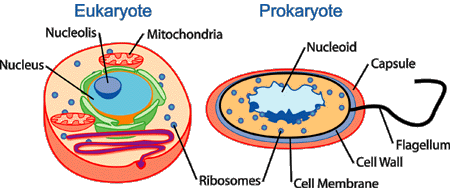
\includegraphics[width=0.6\linewidth]{images/Celltypes.png}
    \caption[Schéma cellules eucaryotes et procaryotes]{Schéma représentant une cellule eucaryote (à gauche) et une cellule procaryote (à droite). La cellule eucaryote est identifiable par un noyau entouré d'une membrane (\textit{Nucleus}), ainsi que par la présence de mitochondries, de petits organites responsables de fournir de l'énergie chimique à la cellule. En revanche, dans la cellule procaryote, le matériel génétique (nucléoïde) est librement dispersé dans le cytoplasme, sans être isolé par une membrane. Crédit image : Creative Commons.}
    \label{fig:cell_types}
\end{figure}

Le développement de la biologie moléculaire a permis d'affiner et de corriger les classifications précédentes en analysant la physiologie et la biochimie des cellules procaryotes, ainsi que les séquences d'ADN des génomes. C'est notamment en étudiant les gènes codant l'ARN 16S, que Carl Woese mis en évidence en 1977, que l'ensemble des procaryotes ne formait pas un groupe monophylétique, mais qu'ils étaient séparés en deux domaines, Bactérie et Archée \cite{woese_phylogenetic_1977}. Longtemps considéré comme des bactéries extrémophiles, il est aujourd'hui clair que les archées représentent un domaine à part entière avec toute sa singularité, comme la composition de leur membrane par exemple \cite{albers_archaeal_2011}. Malgré toute la fascination que nous pouvons avoir pour les archées, et que toutes les méthodes qui seront présentées peuvent s'appliquer aux espèces Archée, nous ne présenterons que très peu de résultats les concernant. C'est pourquoi dans la suite, même si nous parlerons de procaryote, nous considérerons plutôt les bactéries avec un prolongement possible aux archées.

\section{Taxonomie des procaryotes : un problème non résolu ?}

La classification des procaryotes et la définition d'espèce procaryote ne fait pas consensus dans la communauté des microbiologistes. Toutefois, les méthodes de classification se basent sur le même principe de relation entre les individus \cite{aldhebiani_species_2018}. Ces relations peuvent être soit phénétiques, \textit{i.e.}, reposant sur la similarité d'un trait, sans s'intéresser au lien évolutif qui pourrait les relier, soit phylogénétiques, \textit{i.e.}, reposant sur l'hérédité du caractère indépendamment de son état actuel.

Les premières tentatives de classification des bactéries reposaient sur des approches phénétiques, utilisant des critères basés sur les caractéristiques observables de ces organismes : morphologie, physiologie et biochimie.
D'un point de vue morphologique, les microbiologistes examinaient des paramètres tels que la taille des cellules, leur mode de croissance et leur capacité à former des agrégats spécifiques (\autoref{fig:morpho}). La présence ou l'absence de structures spécialisées, telles que les flagelles, était également un critère de différenciation. 
Les caractéristiques physiologiques permettaient, quant à elles, de classer les bactéries selon leur mode de vie, leurs mécanismes métaboliques (anabolisme et catabolisme) et leurs réponses aux conditions environnementales.
L'étude de la composition cellulaire offrait par ailleurs de nouveaux outils pour affiner ces classifications sur le plan biochimique. Par exemple, la coloration de Gram, méthode emblématique, permet de différencier les bactéries en deux grands groupes : les Gram-positives, caractérisées par une paroi épaisse de peptidoglycane, et les Gram-négatives, qui présentent une paroi plus fine associée à une membrane externe lipidique.
Enfin, selon le contexte d’étude, d'autres critères peuvent être intégrés. Dans le domaine médical, la pathogénicité (capacité à induire une maladie) et le sérogroupage (basé sur la composition antigénique de la capsule bactérienne) sont particulièrement utilisés pour identifier et classifier les bactéries d'intérêt clinique.

\begin{figure}[htbp]
    \centering
    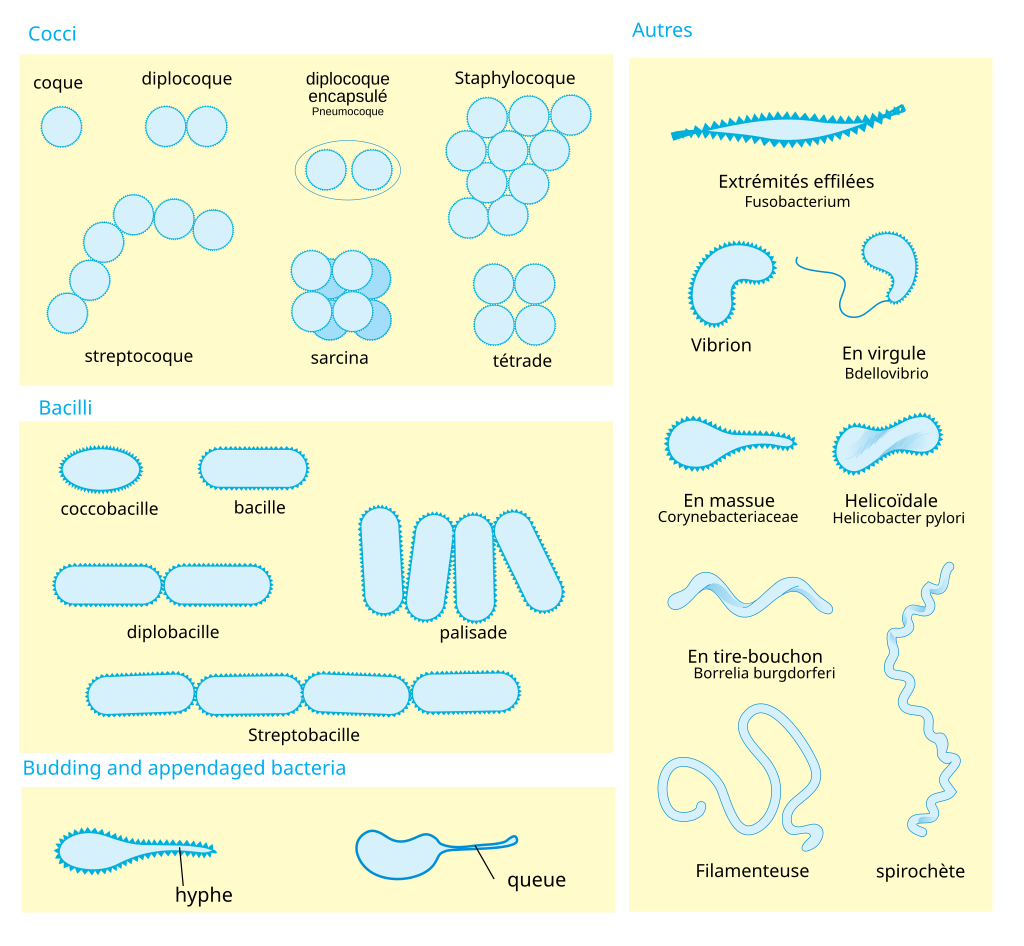
\includegraphics[width=0.75\textwidth, keepaspectratio]{images/Bacterial_morphology_diagram-fr.png}
    \caption[Morphologie et arrangement cellulaire procaryote]{Diversité morphologique des cellules procaryotes et leur arrangement. Par Mariana Ruiz Villarreal \url{https://commons.wikimedia.org/w/index.php?curid=9908634}}
    \label{fig:morpho}
\end{figure}

Avec l'arrivée de la génomique, du séquençage et de la bioinformatique, ces classifications ont peu à peu laissé leur place à des classifications basées sur la phylogénie. Néanmoins, l'ADN a aussi été utilisé comme un critère phénétique définissant des critères biochimiques comme similarité entre les souches. 
Dans ces critères, il y a d'abord le pourcentage de guanine-cytosine (GC) qui permet de différencier 2 souches appartenant à 2 genres différents si elles possèdent plus de 10 mol \%\footnote{1 équivalent molaire équivaut à 100 \% en mole, donc 10 \% en mole équivaut à 0,1 équivalent molaire.}, mais il faut noter qu'une composition en GC proche n'implique pas forcément que les souches soient proches. 
Une approche visant à définir formellement une espèce procaryote a été adoptée en 1987 par un comité d'expert \cite{moore_report_1987}. Il propose que des souches appartiennent à une même espèce si l'ADN s'hybride\footnote{Appariement de 2 brins d'ADN par complémentarité des bases} a plus de 70 \% et que le $\Delta T_m$\footnote{température à laquelle la moitié de l'ADN est dénaturés} diffère de 5 degrés ou moins.

Toutes ces approches ont permis de classer les procaryotes en taxons et dans la nomenclature actuelle, il reste des traces de ces méthodes. Elles sont d'ailleurs toujours utilisées et font partie des traits visibles dans les classifications. Il faut d'ailleurs souligner qu'il n'est pas toujours possible d'obtenir des génomes de bonne qualité pour réaliser des phylogénies.

\section{Espèce procaryote : génomique et phylogénie peuvent-elles trancher ?}

Les approches phénétiques présentées précédemment ont l'intérêt de s'appliquer au laboratoire et donc de regrouper et d'identifier les souches directement. Néanmoins, elles restent relativement approximatives et sont parfois coûteuses (en temps et en moyens). De plus, même si elles répondent aux problèmes de la taxonomie, et donc de ranger les bactéries dans des taxons, elles ne répondent pas à la question du lien entre les différents taxons et comment représenter ce lien, \textit{i.e.}, à la question de la systématique. 

Pour pallier les limites des approches précédentes, une nouvelle méthode a été développée et reste encore largement utilisée en routine aujourd'hui : la comparaison des souches à partir d'un gène marqueur. Il s'agit d'un gène présentant des variations spécifiques parmi les différentes souches d'intérêt, toutes dérivant d'une forme ancestrale commune ayant évolué différemment au fil du temps. Ainsi, le gène marqueur reflète à la fois la similarité entre les souches, permettant leur regroupement, et les événements dits de spéciation ayant conduit à leur séparation en espèces distinctes. On va privilégier l'utilisation de gènes hautement exprimés qui assurent une fonction essentielle à la vie de l'organisme : les gènes de ménage (\textit{house-keeping genes}). Un gène marqueur en particulier est utilisé : l'ADNr 16S, qui a la particularité d'être présent chez tous les procaryotes. En 2007, un arbre du vivant de toutes les espèces a été reconstruit à partir d'un arbre d'ADNr 16S comprenant toutes les souches types séquencées d'espèces de bactéries et d'archées publiées jusqu'à la fin de l'année 2007 \cite{yarza_all-species_2008}. 
En allant encore plus loin, des analyses \textit{multilocus sequence analysis} MLSA ont été proposées \cite{glaeser_multilocus_2015}. Ces analyses prennent en compte plusieurs gènes marqueurs pour réaliser la taxonomie. L'utilisation de plusieurs gènes augmente le niveau d'information et réduit les biais. Toutefois, il n'y a pas de recommandation universelle pour réaliser l'analyse et chaque MLSA est réalisé en fonction des souches de départ. La sélection des gènes et leur nombre sont des paramètres qui ont un impact encore peu évalué sur la taxonomie. Il en va de même pour la taille des fragments considérés pour chaque gène, qui ne représente qu'une partie de la séquence du gène. Enfin, expérimentalement, il est souvent difficile, voire impossible, de concevoir des amorces facilitant l'amplification des gènes dans toutes les souches prises en compte. Malgré ces critiques, l'utilisation de gènes marqueurs est encore aujourd'hui utilisée, mais est peu à peu remplacée par des méthodes prenant en compte l'ensemble du génome.

Le développement des techniques de séquençage d'ADN, initié par F. Sanger en 1977 et sa méthode éponyme \cite{sanger_dna_1977}, ont permis de séquencer les premiers génomes\footnote{le premier génome séquencé est celui du virus de bactérie MS2 \cite{fiers_complete_1976}}. Le premier génome complet procaryote (aussi le premier génome complet d'un organisme cellulaire), celui de la bactérie \textit{Haemophilus influenza}\footnote{Bactérie pathogène, responsable de maladie respiratoire ou de méningites et bactériémie.}, est séquencé en 1995 \cite{fleischmann_whole-genome_1995}. Au début des années 2000 et avec les nombreux projets autour du séquençage et de l'analyse des génomes, comme le projet génome humain \cite{lander_initial_2001}, les technologies de séquençage sont de plus en plus précises et de moins en moins coûteuses, amenant dans la génomique "moderne" : une augmentation exponentielle du nombre de séquences et des séquences plus longues et de meilleure qualité \cite{hugenholtz_prokaryotic_2021,hu_next-generation_2021}. C'est l'arrivée du \textit{Whole Genome Sequencing} (WGS) et de l'analyse de génomes complets de procaryote. Bien que les technologies de séquençage progressent, il faut aussi que les technologies et les algorithmes bioinformatiques se développent à leur tour (vitesse de calcul, gestion des données\dots), pour les utiliser en génomique comparée et en phylogénie, c'est pourquoi les méthodes présentées précédemment étaient privilégiées.

Grâce aux nouvelles méthodes de génomique comparée, que nous présenterons dans le \autoref{chap:comp}, il est désormais possible de considérer le génome complet dans les approches d'assignation taxonomique d'organismes. Une de ces approches est l'\textit{Average Nucleotide Identity} (ANI), qui rend compte de la similarité entre 2 séquences nucléotidiques. Le score d'ANI va d'ailleurs remplacer celui de l'hybridation, où un ANI inférieur 95 \% permet de différencier les espèces à la place d'une hybridation à 70 \% \cite{goris_dnadna_2007}. Plus récemment, le seuil de 95 \% a été confirmé par les auteurs de FastANI \cite{jain_high_2018}, utilisant plus de 90 000 génomes. Ils ont montré l'existence d'un \textit{gap}, espace où l'ANI diminue fortement avant 95 \% (\autoref{fig:ANI_gap_sp}).


\begin{figure}[htbp]
    \centering
    % Première image
    \subfloat{%
        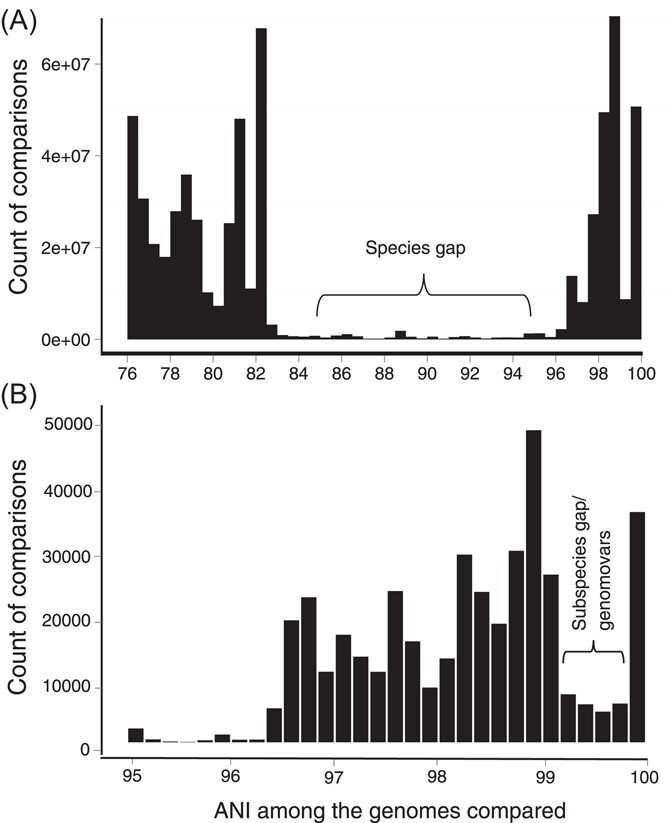
\includegraphics[width=0.5\textwidth]{images/ANI_gap.jpg}
    }
    \hfill % Espace flexible entre les deux images
    % Deuxième image
    \subfloat{%
        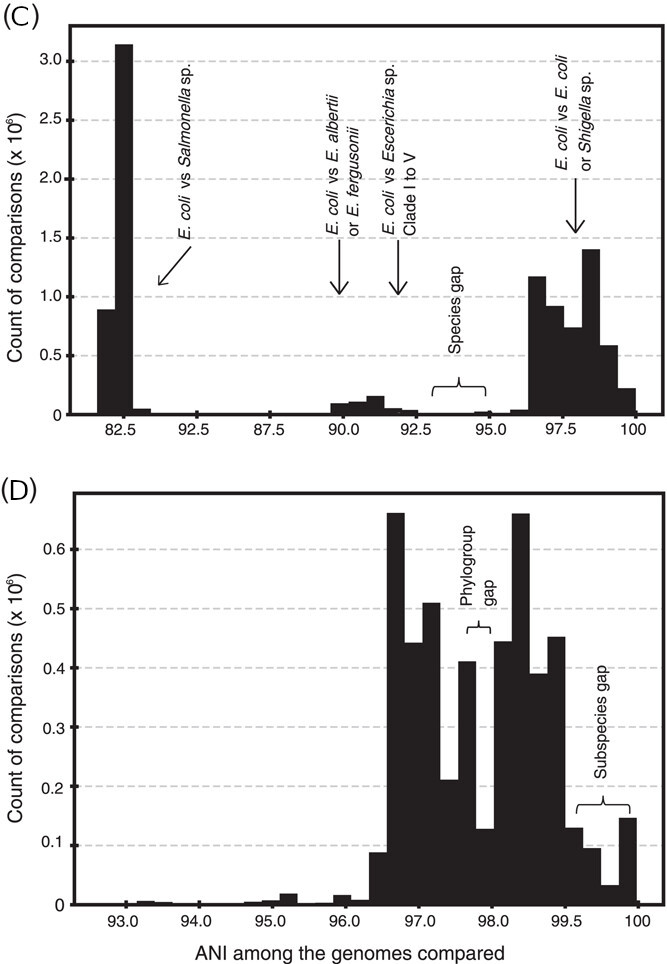
\includegraphics[width=0.44\textwidth]{images/ANI_sp.jpg}
    }
    \caption[Variation du score d'ANI au niveau de l'espèce]{Variation du score d'ANI au niveau de l'espèce. (A-B) Les histogrammes sont basés sur des comparaisons par paire effectuées avec FastANI. (A) Le Score d'ANI représenté au niveau de l'espèce se base sur les données de Jain \textit{et al}. On y retrouve un \textit{gap} entre 84 et 95 \% d'ANI. (B) Score d'ANI représenté au niveau intra-espèce sur les données de Rodrigues-R \textit{et al}. On retrouve un \textit{gap} entre 99,2 et 99,8 \% d'ANI. (C-D) Score d'ANI au niveau du groupe \textit{Escherichia coli}. Le nombre de génomes utilisés est le suivant : \textit{E. coli} : 2815 ; \textit{Salmonella enterica} : 1351 ; \textit{Escherichia fergusonii} : 57 ; \textit{Escherichia albertii} : 70 ; et \textit{Shigella flexneri} : 93 (tous les génomes complets disponibles au NCBI en juillet 2023). (C) Comparaison de l'ANI entre \textit{E.Coli} et d'autres espèces. Le seuil de 95 \% délimitant l'espèce est retrouvé. Un \textit{gap} à 97 \% existe entre \textit{E.coli} et \textit{Shigella flexneri} (une espèce d'\textit{E.Coli} particulière pour ces propriétés infectieuse). (D) Analyse de l'ANI au sein des génomes de \textit{E.Coli}. L'écart d'ANI de 99,5 \% est aussi prononcé, par rapport aux barres adjacentes, que l'écart d'ANI de 98 \%-97 \% qui correspond à l'écart entre les phylogroupes d'\textit{E. coli}, un groupe distinct et bien reconnu au sein d'\textit{E. coli}. Figures et légende adaptées de \cite{konstantinidis_sequence-discrete_2023}}
    \label{fig:ANI_gap_sp}
\end{figure}


Pourtant, la communauté n'est toujours pas arrivée à un consensus sur la classification des procaryotes en espèces et même sur l'existence d'espèces procaryotes. On peut d'abord critiquer l'approche et les résultats des études utilisant l'ANI, qui se limitent aux génomes de bonne qualité et complets, ce qui \textit{de facto} limite le nombre de génomes et d'espèces potentielles pris en compte, tout en augmentant la redondance et limitant la diversité et la variabilité. De plus, la démarche apporte le biais d'utiliser une taxonomie déjà existante. Il faut aussi prendre en compte que la dynamique évolutive des procaryotes, que nous détaillerons dans le chapitre suivant (\autoref{sec:dyn_evo}), n'est pas linéaire et héréditaire, mais que les procaryotes sont capables de recevoir et d'échanger de l'ADN. C'est pourquoi des auteurs soutiennent une définition plus écologique de l'espèce procaryote \cite{luo_genome_2011}, prenant en compte ces échanges agissant sur la \textit{fitness} des organismes dans leur environnement.


On peut donc convenir qu'il n'est pas encore communément admis de parler d'espèce procaryote. Il existe toutefois des caractéristiques communes et spécifiques aux procaryotes ainsi que des traits propres à chaque taxon. De nombreuses méthodes et démarches scientifiques parviennent à construire une phylogénie des procaryotes, mais celle-ci doit être replacée dans son contexte d'étude pour prendre sens. Notamment dans les travaux de recherches que j'ai réalisés, où il était nécessaire de se baser sur une classification des génomes en espèce. Dans le contexte de nos travaux, la similarité des séquences l'emporte comme critère de classification, nous utiliserons donc des génomes provenant de bases de données utilisant des critères comme l'ANI ou des gènes marqueurs pour construire des pangénomes.

%Enfin, avec l'explosion du nombre de séquences disponible, nous voyons l'émergence d'un paradoxe : de plus en plus de données sont disponibles, mais alors que l'on pensait pouvoir ranger les procaryotes dans des boites bien précises qui se verraient valider au cours du temps, une nouvelle exception vient renverser l'ordre actuel et la phylogénie doit être revue.

\section{Systématique : l'homologie et ses déclinaisons}

Les méthodes présentées ci-dessus, sont  des aides précieuses pour convenir d'une taxonomie des procaryotes, mais aussi pour étudier leur évolution au cours du temps et retracer l'origine et l'histoire des gènes. Il reste donc à lier et à représenter le lien entre les gènes. 

Une première approche intuitive est de rechercher une origine commune entre les gènes, appelé gène ancestral. Si un tel gène existe, on dit que les gènes issus de ce gène ancestral sont homologues. Dans un second temps, il convient d'étudier les évènements évolutifs qui ont conduit à la séparation des gènes pour préciser le type d'homologie (\autoref{fig:homologue}). 
Le premier évènement est un évènement dit de spéciation et conduit à l'émergence d'une espèce. Dans ce cas, si les gènes sont uniquement séparés par des spéciations, on dit qu'ils sont orthologues. Le second évènement est une duplication des gènes sur le même génome (cf. \autoref{sec:rearragement}). Les gènes sont alors dits paralogues et vont évoluer de façon indépendante dans le génome. Un autre évènement évolutif, fréquent chez les procaryotes, est celui du transfert horizontal, \textit{i.e.}, l'échange de matériel génétique entre organismes (cf. \autoref{sec:evo_hz}). Lorsque des gènes sont transférés horizontalement, ils sont dits xenologue.

\begin{figure}[htbp]
    \centering
    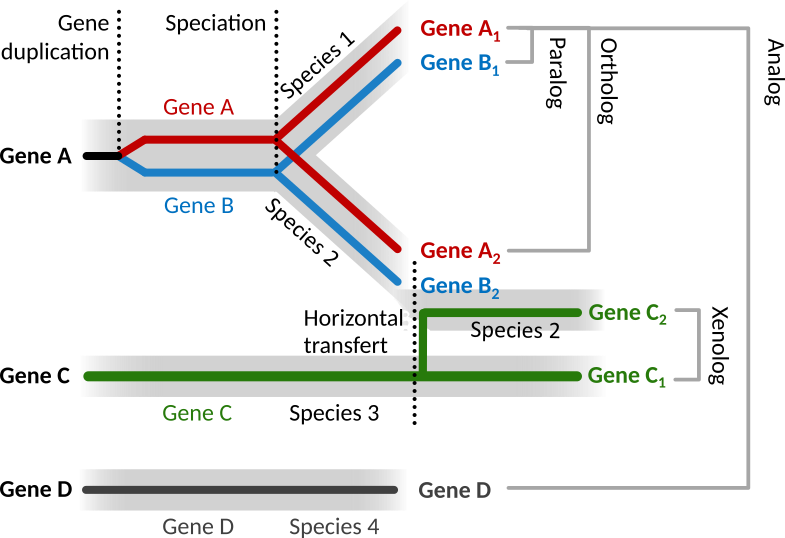
\includegraphics[width=.9\textwidth]{images/homologs.png}
    \caption[Schéma représentatif des différents types d'homologie]{Schéma représentatif des différents types d'homologie. Figure extraite et adaptée de \url{https://en.m.wikipedia.org/wiki/Sequence_homology} sous licence Creative Common}
    \label{fig:homologue}
\end{figure}

Toutes ces notions sont essentielles pour poser des hypothèses de travail qui seront utilisées dans les analyses de génomique comparée \cite{koonin_orthologs_2005,stamboulian_ortholog_2020}. Une de ces hypothèses que nous utiliserons dans nos analyses est celle que des gènes homologues vont coder pour des fonctions similaires\footnote{\textit{N.B} : 2 gènes codant pour la même fonction ne sont pas nécessairement homologues. Il existe des cas de convergence évolutive, \textit{i.e.}, une fonction similaire sans origine commune. Il est aussi possible que des séquences courtes ou peu complexe semble homologue, mais cette apparente homologie serait liée au hasard.}. Plus précisément, on suppose que des gènes orthologues vont coder pour une même fonction et vont donc faire également partie du même processus. Les gènes paralogues peuvent avoir des fonctions différentes, mais qui reste proche, par exemple pour des enzymes, le substrat va changer, mais la réaction rendra un produit chimiquement proche \cite{mirny_using_2002}.